\chapter{Question4}
\section{问题概述}
%
%%对问题的直观描述
%
本问题要求实现基于期望的智能体,它能够较好地处理对手为并不保证按照最优解执行的智能体的情况。
%
%对项目已有代码的阅读和理解
%
%
%解决问题的思路和想法
%
\section{算法设计}
%
%用自己的语言描述解决问题所使用的算法的原理及功能,设计思路和算法流程图
%
本问题中假设幽灵是随机移动的。对于这种情况,Minimax算法不再适用,因为对手不再保证执行最优解。对此,应该调整正方,即吃豆人,选择下一步
的策略。在Minimax算法中,选择的依据是“对手总是选择最优解”这一前提,而此时,对手的操作是完全随机的,即任何一个合法操作都等概率被执行。将这些
操作的效果综合起来,便是分数的期望,因此,正方选择操作的依据是使得分数的期望最大化。
\begin{algorithm}[h]
    \SetKw{maximize}{maximize} 
    dummy,action = \maximize(gameState,1)\tcp*[h]{这里无需返回的分数}\;
    \Return{action}
    \caption{Minimax(gameState)}
\end{algorithm}

\begin{procedure}[h]
    \KwOut{bestScore,bestAction}
    \SetKw{in}{in}
    \SetKw{randomMove}{randomMove}
    \tcp*[h]{给定状态和对应深度,返回从当前状态出发所能达到的最佳分数和对应的动作}\;
    actions = gameState.getLegalActions()\;
    ghostNum = gameState.getNumAgent - 1\;
    \If{depth > depthLimit or actions == None}
    {\Return{evaluationFunction(gameState),None}\tcp*[h]{无法继续行动,直接返回当前状态的分数}}
    bestScore = $-\infty$\;
    bestAction = None\;
    \ForEach{action \in actions}
    {
        next = gameState.generateSuccessor(gameState,action)\tcp*[h]{获取下一个状态}\;
        score = \randomMove(next,1,ghostNum,depth)\;
        \If{score > bestScore}
        {
            bestAction = action\;
            bestScore = score\;
        }
    }
    \Return{bestScore,bestAction}
    \caption{maximize(gameState,depth)}
\end{procedure}

\begin{procedure}[h]
    \KwOut{bestScore,bestAction}
    \SetKw{in}{in}
    \SetKw{len}{len}
    \SetKw{randomMove}{randomMove}
    \tcp*[h]{给定状态和对应深度,返回从当前状态出发所能达到的最佳分数和对应的动作}\;
    actions = gameState.getLegalActions()\;
    \If{depth > depthLimit or actions == None}
    {\Return{evaluationFunction(gameState),None}\tcp*[h]{无法继续行动,直接返回当前状态的分数}}
    totScore = 0\;
    \ForEach{action \in actions}
    {
        next = gameState.generateSuccessor(gameState,action)\tcp*[h]{获取下一个状态}\;
        \eIf{ghostNo == ghostNum}
        {
            score,dummy = \maximize(next,depth+1)\tcp*[h]{当前智能体是最后一个幽灵,下一层为吃豆人}
        }
        {
        score = \randomMove(next,ghostNo+1,ghostNum,depth)
        }
        totScore += score\;
    }
    \Return{totScore/ \len(actions)}\tcp*[h]{等概率时期望便是平均值}\;
    \caption{randomMove(gameState,ghostNo,ghostNum,depth)}
\end{procedure}
\section{算法实现}
\begin{lstlisting}[emph={[3]currentGameState,gameState,depth,alpha,beta,ghostNo,ghostNum},emphstyle={[3]\color{vscode_parametercolor}},emph={[4]GameState,MinimaxAgent,AlphaBetaAgent},emphstyle={[4]\color{vscode_classcolor}}]
class ExpectimaxAgent(MultiAgentSearchAgent):
    def maximize(self, gameState: GameState, depth: int):
        actions = gameState.getLegalActions(0)
        if gameState.isWin() or depth > self.depth or not actions:
            return self.evaluationFunction(gameState), None
        bestScore = -float('inf')
        bestAction = None
        for action in actions:
            next = gameState.generateSuccessor(0, action)
            score = self.randomMove(next, 1, gameState.getNumAgents() - 1, depth)
            if score > bestScore:
                bestAction = action
                bestScore = score
        return bestScore, bestAction

    def randomMove(self, gameState: GameState, ghostNo: int, ghostNum: int, depth: int):
        actions = gameState.getLegalActions(ghostNo)
        if gameState.isLose() or not actions:
            return self.evaluationFunction(gameState)
        totScore = 0
        for action in actions:
            next = gameState.generateSuccessor(ghostNo, action)
            if ghostNo == ghostNum:
                score, _ = self.maximize(next, depth + 1)
            else:
                score = self.randomMove(next, ghostNo + 1, ghostNum, depth)
            totScore += score
        return totScore / len(actions)

    def getAction(self, gameState: GameState):
        return self.maximize(gameState, 1)[1]
\end{lstlisting}
\section{实验结果}
%
%对试验结果进行详细展示,对每个问题展示测试截图,对于测试用例进行描述说明,对于为通过测试的用例结合自己的算法进行分析,可以结合调试过程进行分析
%
我成功获得了本问题的所有分数,图\ref{q4}为实验结果。所用到的测试用例中,expectimax测试是特有的,测试的是该算法的基本功能。
\begin{figure}[H]
    \centering
    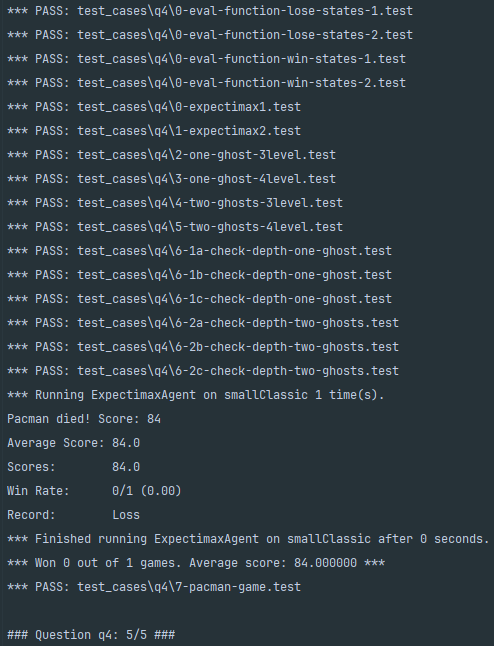
\includegraphics[scale = 0.7]{pic/q4.png}
    \caption{Question4实验结果}\label{q4}
\end{figure}
%
%在算法原理的基础上,结合代码,讲述算法的实现细节、和兴函数、模块输入输出,数据结构定义等内容
%
%
%对试验结果进行详细展示,对每个问题展示测试截图,对于测试用例进行描述说明,对于为通过测试的用例结合自己的算法进行分析,可以结合调试过程进行分析
%
%实验中遇到的问题及解决方案,收获和思考:对算法的理解、优缺点的评价、算法的适用场景
%
